\chapter[Система команд. Управление ветвлениями. Системные вызовы]{Семинар 03. Система команд. Методы адресации. Ветвления и переходы. Системные вызовы}

Целью семинара является знакомство с организацией регистров и памяти эмулятора процессора RISC-V, использованием методов адресации для работы с памятью. Помимо этого предполагается более детальное изучение работы отладчика, а также мониторинга регистров и памяти. Основны вопросы, которые предполагается рассмотреть на семинаре.


\begin{enumerate}
    \item Организация команд. Cистема команд.
    \begin{itemize}
        \item Форматы команд. Общая идея предложенных форматов.
        \item Мнемоника команд.
        \item Псевдокоманды.
    \end{itemize}
    \item Область кода.
    \begin{itemize}
        \item Методы адресации данных, используемые в ассемблере RISC-V.
        \item Моделирование на ассемблере различных операторов управления.
    \end{itemize}
    \item Имитация в эмуляторе системных вызовов. Аналогии системных вызовов в операционных системах.
    \item Примеры простых целочисленных алгоритмов.
\end{enumerate}

\section{Сценарий семинара}

\subsection{Организация команд. Cистема команд}
Кратко (по сути как повтор общей классификации) определить специфику системы команд RISC процессоров и ее отличие от системы команд CISC процессоров. Также отметить, что для семейства RISC-V существуют различные системы команд в зависимости от разрядности процессоров и их дополнительного обвеса. Но имеется общая специфика, связаннай с построением форматов и размером команд (32 разряда)

\subsubsection{Форматы команд. Общая идея предложенных форматов}
Привести и пояснить (достаточно кратко) основные форматы команд 32-разрядной версии процессора (RV32I). Рассмотреть четыре базовых типа команд (рисунок~\ref{command-01}):
\begin{itemize}
    \item \textbf{R} --- типа «регистр-регистр-регистр» (Register)
    \item \textbf{I} --- типа «непосредственное значение-регистр-регистр» (Immediate)
    \item \textbf{S} --- типа «регистр-регистр-непосредственное значение» (Store)
    \item \textbf{U} --- типа «непосредственное значение-регистр» (Upper)
\end{itemize}

\begin{figure}[htbp]
    \centering
    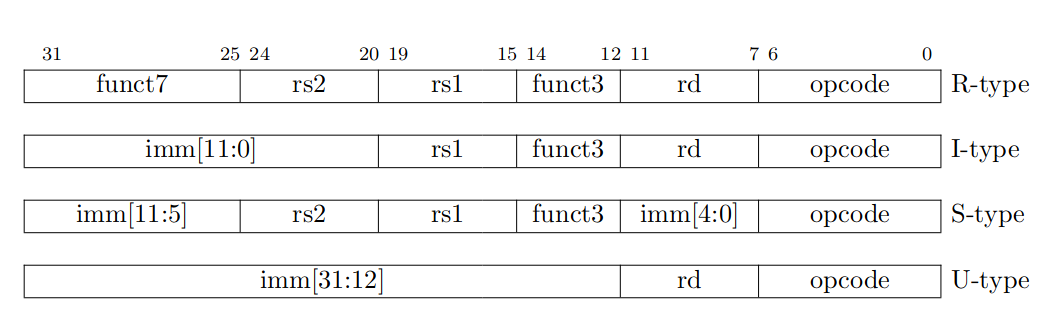
\includegraphics[width=1.0\textwidth]{img/RISCV_4_Commands.png}
    \caption{Основные форматы команд 32-разрядного процессора RISC-V}
    \label{command-01}
\end{figure}
Обозначения на рисунке:
\begin{itemize}
    \item \textbf{opcode} — код операции (6 битов)
    \item \textbf{rs1} --- № регистра-источника (5 битов)
    \item \textbf{rs2} --- № регистра-операнда (5 битов)
    \item \textbf{rd} --- № регистра-приёмника (5 битов)
    \item \textbf{imm[11:0]} --- непосредственный операнд размером в 12 битов (В случае, когда непосредственное значение определяет «приёмник» (смещен адреса для «близкого» перехода или записи результата в память), 12 битов целиком в поле rd не помещаются, и его приходится «распиливать» (инструкция типа S). Непосредственный операнд всегда знаковый, и его знак всегда приходится на 31-й бит)
    \item \textbf{imm[31:12]} --- непосредственный операнд размером в 20 битов. Используется в инструкциях типа U для заполнения старших двадцати битов регистра (в операциях «далёкого» перехода и как дополнительная инструкция при записи в регистр полного 32-разрядного непосредственного операнда)
    \item \textbf{funct} --- поле функции (6 битов), используется для разных инструкций, у которых код операции одинаковый. Например, все арифметические инструкции типа I имеют одинаковый opcode OP-IMM (чему он равен?), а различаются полем funct. По-видимому, для эффективной реализации R-команд в конвейере удобнее не декодировать опкод, а по-быстрому сравнить его с нулём, и получать значения регистров, параллельно декодируя функцию, чтобы потом её применить.
\end{itemize}

\subsubsection{Мнемоника команд}

Изначально мнемонику команд можно рассмотрить в системе помощи RARS (раздел Basic Inctructions), где в алфавитном порядке представлены практически все команды. Однако этот формат не вполне удобен для постепенного изучения. Поэтому можно сослаться на пару таблиц, в которых команды систематизирован, но представлены без описания. Можно предложить совместное использование этой справочной информации по мере необходимости. В принципе в методе по самостоятельной работе данный материал стоит систематизировать и выложить в LMS. Начало положено. Там можно сделать все в соответствии с порядком изучения.
Обе таблицы с кратким представлением набора команд (\verb|RARS_reference_card.pdf| и \verb|riscv-reference-card.pdf|) я положил в каталог \verb|info| на \verb|gitflic|.

\subsubsection{Псевдокоманды}

Рассмотрение мнемоники псевдокоманд в целом можно осуществить по той же схеме, что и изучение команд. Их достаточно обширный список представлен в системе помощи. Однако, в связи с тем, что речь идет о первоначальном знакомстве, вряд ли имеет смысл на этой мнемонике долго останавливаться. Также можно обратиться к отображениям в дополнительной информации. Или к методическим материалам для самостоятельного изучения (надеюсь, что соответствующие материалы и презентации разработаем).

\section{Область кода}

Можно еще раз подчеркнуть адресное пространство, в котором располагается программный код. Также отметить, что при описании на ассемблере соответствующими директивами (\verb|.data| и \verb|.text|) можно чередовать код и данные, а ассемблер разместит их в своих областях.

\subsection{Методы адресации данных, используемые в ассемблере RISC-V}

Пояснить основные методы адресации, которые используются в процессоре на уровне обмена с памятью. Показать необходимость использования адресации в памяти как для обращения к данным и их пересылки, так и для организации управления вычислениями.

\subsubsection{Ветвления и переходы}

Можно рассмотреть базовые инструкции вида <<сравнить и перейти>> \\ (\verb|beq/bne /blt/bge/btlu/bgeu|. Все остальные инструкции вида \verb|b*|, включая безусловный переход \verb|b| --- это псевдоинструкции, потому что получаются простой перестановкой регистров--операндов или подстановкой регистра \verb|zero| в нужное место. Непосредственный 12-битный операнд используется для хранения смещения относительно текущего адреса. Вычислением этого смещения из метки занимается ассемблер, оно бывает положительное (вперёд) и отрицательное (назад, как в примере). 12 битов хватает на то, чтобы сделать переход на 4 килобайта кода (4, а не 2, потому что адрес всегда кратен 2 и самый младший бит просто не хранится).

Пример перехода по постусловию (из материалов Курячего):
\begin{verbatim}
    # Переходы по постусловию
    li      s2 10           # Граница счётчика
    li      s1 1            # Счётчик
    loop:   li      a7 1            # Вывод счётчика
    mv      a0 s1
    ecall
    addi    s1 s1 1         # Увеличение
    blt     s1 s2 loop      # Сравнение счётчика и границы и переход
    li      a7 10           # Останов
    ecall
\end{verbatim}
Можно рассмотреть, что получится после компиляции и выделить непосредственные 12--разрядные операнды

Пример перехода по предусловию с длинным переходом (из материалов Курячего):
\begin{verbatim}
    li      s2 10
    li      s1 1            # Инициализация
    loop:   bge     s1 s2 final     # Проерка условия
    li      a7 1            # Тело
    mv      a0 s1
    ecall                   # Вывод целого
    li      a7 11
    li      a0 10
    ecall                   # Вывод перевода строки
    addi    s1 s1 1         # Изменение
    j       loop            # Дополнительный переход
    final:  li      a7 10
    ecall\end{verbatim}
Безусловный переход может называться b, а может j — это одна и та же псевдоинструкция. Это инструкция <<длинного>> перехода типа J (20 битов, т. е. по мегабайту в обе стороны с учётом ещё одного младшего бита). Есть более подробное описание у Курячего. Но думаю, что сильно на данном этапе заморачиваться не стоит, так как пока программы простые. А в методических указаниях можно более подробно описать. Возможно, что данный пример можно пока тоже не рассматривать...

\subsubsection{Косвенная адресация и массивы}

Как вариант доступа к данным --- записать полный абсолютный адрес в регистр, и воспользоваться инструкцией, которая работает с памятью, находящейся по этому адресу. Пример использования псевдоинструкции \verb|lw метка| (из Курячего):
\begin{verbatim}
    .data
    .word   0x1223344
    var:    .word   0xdeadbeef
    addr:   .word   var
    .text
    lw      t1 var
    lw      t2 addr
    lw      t3 (t2)
    lw      t4 4(t2)
    lw      t5 -4(t2)
\end{verbatim}

Результаты компиляции:
\begin{verbatim}
    Address    Code        Basic                     Source

    0x00400000  0x0fc10317  auipc x6,0x0000fc10   6   lw      t1 var
    0x00400004  0x00432303  lw x6,0x00000004(x6)
    0x00400008  0x0fc10397  auipc x7,0x0000fc10   7   lw      t2 addr
    0x0040000c  0x0003a383  lw x7,0x00000000(x7)
    0x00400010  0x0003ae03  lw x28,0x00000000(x7) 8   lw      t3 (t2)
    0x00400014  0x0043ae83  lw x29,0x00000004(x7) 9   lw      t4 4(t2)
    0x00400018  0xffc3af03  lw x30,0xfffffffc(x7) 10  lw      t5 -4(t2)
\end{verbatim}
\begin{itemize}
    \item Инструкция \verb|auipc| формирует в регистре \verb|t1| (он же \verb|x6|) адрес, по которому лежит интересующее нас значение.
    \item далее \verb|lw| выбирает это значение из памяти, попутно скорректировав его смещением 4, и кладёт в тот же регистр \verb|t1|.
    \item По метке \verb|addr| размещается метак \verb|var|, то есть адрес \verb|0x10010004|.
    \item Он оказывается в регистре \verb|t2| тем же способом, каким \verb|0xdeadbeef| оказалось в \verb|t1|.
    \item После этого с помощью явно указанного смещения в инструкции \verb|lw| получаем в разных регистрах содержимое памяти по адресам \verb|0x10010004|, \verb|0x10010008| и \verb|0x10010000| сооответственно.
\end{itemize}

Косвенная адресация — единственный способ обработки массива. Массив — это адрес в памяти и длина (количество элементов * размер одного элемента). В примере массив слов расписывается последовательными значениями:
\begin{verbatim}
    .data
    array:  .space  64
    arrend:
    .text
    la      t0 array
    la      t1 arrend
    li      t2 1
    loop:   sw      t2 (t0)
    addi    t2 t2 1
    addi    t0 t0 4
    bltu    t0 t1 loop
    li      a7 10           # Останов
    ecall
\end{verbatim}
Пояснить каким образом формируется адрес текущего элемента массива. Также акцентировать внимание, что остановка осуществляет не по числу элементов в массиве (что тоже возможно), а по достижению адреса \verb|arrend|, фиксирующего ячейку после завершения массива.

\subsection{Моделирование на ассемблере различных операторов управления}
Учитывая, что основные элементы и команды управления уже показаны, можно кратко остановиться на примерах имитации базовых операторов управления языков высокого уровня. Думаю, что для понимания достаточно их прогона. Тоже будут в LMS.

\subsubsection{Оператор if}
\begin{verbatim}
    # if (t0 == 0) {
        #     t1 = 1;
        # } else if (t0 < 0) {
        #     t1 = 2;
        # } else if (t0 >= 10) {
        #     t1 = 3;
        # } else {
        #     t1 = 4;
        # }
    main:
    li   a7, 5
    ecall
    mv   t0, a0
    if_0:
    bnez t0, if_less_0
    li   t1, 1
    j    end_if
    if_less_0:
    bgtz t0, if_greater_10
    li   t1, 2
    j    end_if
    if_greater_10:
    li   t3, 10
    ble  t0, t3, else
    li   t1, 3
    j    end_if
    else:
    li   t1, 4
    end_if:
    li   a7, 1
    mv   a0, t1
    ecall
\end{verbatim}

\subsubsection{Оператор while}
\begin{verbatim}
    # while((t0 = read_int()) != 0) {
        #    print_int(t0)
        #    print_char('\n')
        # }
    while:
    li   a7, 5
    ecall
    mv   t0, a0
    beqz a0, end_while
    li   a7, 1
    ecall
    li   a7, 11
    li   a0, '\n'
    ecall
    j    while
    end_while:
\end{verbatim}

\subsubsection{Оператор for}
\begin{verbatim}
    # for (t0 = 0; t0 < t1; ++t0) {
        #     print_int(t0)
        #     print_char('\n')
        # }
    for:
    li   a7, 5
    ecall
    mv   t1, a0
    mv   t0, zero
    next:
    beq  t0, t1, end_for
    mv   a0, t0
    li   a7, 1
    ecall
    li   a7, 11
    li   a0, '\n'
    ecall
    addi t0, t0, 1
    j    next
    end_for:
\end{verbatim}

\section{Имитация в эмуляторе системных вызовов. Аналогии системных вызовов в операционных системах}

Разговор о том, что системные вызовы эмулятора отличаются от системных вызовов ОС идет постоянно, начиная с первого семинара. Поэтому в ходе этого и последующих семинаров дополнительно стоит пояснять только новые вызовы и отсылать к системе помощи эмулятора, в которой хорошо описаны принципы их работы. Поэтому здесь особо акцентироваться не на чем. Только повторять ранее сказанное, избегая при этом занудства...
Может быть не имеет смысла держать этот пункт в теме.

\section{Примеры простых целочисленных алгоритмов}

После рассмотрения команд управления можно рассмотреть пару простых алгоритмов. Ниже представлены в качестве примеров нахождение числа Фибоначчи и вычисление наибольшего общего делителя двух чисел (алгоритм Евклида). В целом заострять внимание на них сильно не стоит в связи с очевидностью решений. Но прогнать их студентам имеет смысл. Возможно, с разными исходным данным, чтобы показать отсутствие обработки некорректных входных данных. Программы также будут находиться в LMS.

\subsection{Вычисление числа Фибоначчи}
\begin{verbatim}
    #
    # Example that calculates the Fibonacci sequence.
    #
    main:
    mv   t0, zero
    li   t1, 1

    li   a7, 5
    ecall
    mv   t3, a0
    fib:
    beqz t3, finish
    add  t2, t1, t0
    mv   t0, t1
    mv   t1, t2
    addi t3, t3, -1
    j    fib
    finish:
    li   a7, 1
    mv   a0, t0
    ecall
\end{verbatim}

\subsection{Алгоритм Евклида}
\begin{verbatim}
    # Calculates the greatest common divisor of
    # two values using the Euclidean algorithm.
    # int gcd(int a, int b) {
        #    while (a != b)
        #        if a > b
        #            a = a - b;
        #        else
        #            b := b - a;
        #    return a;
        # }

    .data
    arg01:  .asciz "Input 1st number: "
    arg02:  .asciz "Input 2nd number: "
    result: .asciz "Result = "
    ln:     .asciz "\n"

    .text
    main:
    la 	a0, arg01   # Подсказка для ввода первого числа
    li 	a7, 4       # Системный вызов №4. Ввод строки в стиле Си
    ecall

    li  a7, 5       # Системный вызов №5. Ввод целого
    ecall
    mv  t1, a0

    la 	a0, arg02   # Подсказка для ввода второго числа
    li 	a7, 4       # Системный вызов №4. Ввод строки в стиле Си
    ecall

    li  a7, 5
    ecall
    mv  t2, a0

    loop:
    beq t1, t2, finish

    slt t0, t1, t2
    bne t0, zero, if_less

    sub t1, t1, t2
    b   loop

    if_less:
    sub t2, t2, t1
    b   loop

    finish:
    la a0, result   # Подсказка для выводимого результата
    li a7, 4        # Системный вызов №4
    ecall

    li  a7, 1 		# Системный вызов №1 — вывести десятичное число
    mv  a0, t1
    ecall

    la 	a0, ln      # Перевод строки
    li  a7, 4       # Системный вызов №4
    ecall

    li      a7 10   # Системный вызов №10 — останов программы
    ecall
\end{verbatim}

\section{Домашнее задание}

\subsection{До 10 баллов}

Разработать на ассемблере RARS программу, осуществляющую целочисленное деление для 32-разрядных целых чисел со знаком, используя операции вычитания, ветвления и циклы. Исходные делимое и делитель вводятся с клавиатуры в десятичной системе счисления. Полученные в результате деления частное и остаток необходимо вывести на консоль эмулятора. Остаток от деления вычисляется по правилам, используемых при выполнения операции вычисления остатка (\verb|%|) в языках программирования \verb|C/C++|. При делении учитывать знаки операндов и результатов, а также возможность ошибок при делении на ноль.

В отчете привести примеры скриншотов консоли, демонстрирующие все возможные комбинации тестового покрытия.

Рекомендации. Предварительно данную программу можно отработать на языках более высокого уровня (рекомендуется использовать C/C++).


